%=========================================================

% Here you can choose to compile with or without solutions.
% However, this definition is ignored if you use any
% command from the `Makefile`.
\providecommand{\withSol}{\iftrue}

%=========================================================

\documentclass
[twoside,english,colorbacktitle,accentcolor=tud9c]
{tudexercise}

\usepackage[T1]{fontenc}
\usepackage[latin9]{inputenc}
\usepackage{amstext}
\usepackage{amsmath}
\usepackage{graphicx}
\usepackage{setspace}
\usepackage{multicol}
\usepackage{mathtools}
\usepackage{dsfont}
\usepackage{units}
\usepackage{subfigure}
\usepackage{color}
\usepackage{booktabs}
\usepackage{fancyref}
\usepackage[ngerman,english]{babel}

%=========================================================

\def\homework{1}
\def\homeworkVer{1}
\def\homeworkSolVer{1}
\def\lecture{Robot Learning}
\def\semester{Winter Semester 2017/2018}
\def\prof{Prof. Dr. J. Peters, D. Tanneberg, M. Ewerton}
\def\deadline{Due date: Wednesday, 15 November 2017 (before the lecture)}

%=========================================================

\ifcsname withSol\endcsname\else
  \expandafter\let\csname withSol\expandafter\endcsname
                  \csname iffalse\endcsname
\fi

\withSol
	\usepackage[solutions]{iasHomework}
\else
	\usepackage{iasHomework}
\fi

%=========================================================

% USE YOUR NAMES!
\newcommand{\studentdata}{}
%\newcommand{\studentdata}{John Doe, 1234567 \qquad Jane Doe, 7654321}

\begin{document}
	
	\hwtitle{}
	\maketitle
	
	\begin{examheader}
		\normalsize
		\vspace{-1em}
		Name, Surname, ID Number \hfill \studentdata{}
		\vspace{-1em}
	\end{examheader} 
	
	\textbf{Markus, Lamprecht, 2424163 \hfill \studentdata{}}
	\textbf{Moritz, Knaust, ???? \hfill \studentdata{}}
	
	%---------------------------------------------
%---------------------------------------------
%---------------------------------------------
%---------------------------------------------
\exercise{Robotics in a Nutshell}
You are considering to buy a new multi-purpose robot platform. Its kinematic chain has two rotational $q_{\{1,3\}}$ and two linear $q_{\{2,4\}}$ degrees of freedom (DoFs), as shown in the figure below. These four joints are actuated with forces and torques of $u_i$, $i\in\{1,2,3,4\}$. A gripper is mounted on the end of the robot, indicated by the letter \textbf{E}. The robot's base is mounted on a table. We assume that the base Cartesian coordinates at the mount are $x_\textrm{base}=[0,0,0]$.  

\begin{center}
   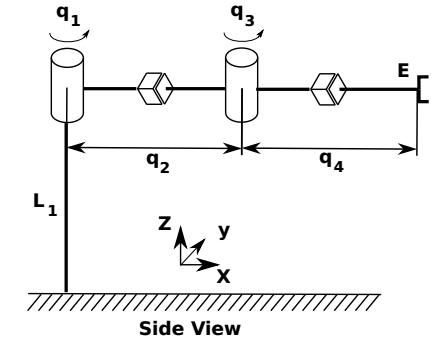
\includegraphics[width=0.35\textwidth]{img/robot.png} 
\end{center}



\begin{questions}

%----------------------------------------------

\begin{question}{Forward Kinematics}{2}
Compute the kinematic transformation in the global coordinate system from the base $\vec{x_\textrm{base}}$ to the end-effector \textbf{E}.  
Write the solution for the $\vec{x_\textrm{end-eff}}=[x,y,z]^T$  according to the joint values $q_i$, where $i \in \{1,2,3,4\}$.

\begin{answer}
	Compute the position with rotation and translation matrices:
	\begin{equation}
		\begin{split}
			H_5 &= Trans_{z,l1}\cdot Rot_{z,q_1}\cdot Trans_{x,q_2}\cdot Rot_{z,q_3}\cdot Trans_{x,q_4}\\
			H_5 &= 
			\begin{pmatrix} 
				1& 0& 0& 0\\
				0& 1& 0& 0\\
				0& 0& 1& L1\\
				0& 0& 0& 1
			\end{pmatrix}
			\cdot
			\begin{pmatrix}
				c_{q_1}& -s_{q_1}& 0& 0\\
				s_{q_1}& c_{q_1}& 0& 0\\
				0& 0& 1& 0&\\
				0& 0& 0& 1&
			\end{pmatrix}
			\cdot
			\begin{pmatrix} 
				1& 0& 0& q_2\\
				0& 1& 0& 0\\
				0& 0& 1& 0\\
				0& 0& 0& 1
			\end{pmatrix}
			\cdot
			\begin{pmatrix}
				c_{q_3}& -s_{q_3}& 0& 0\\
				s_{q_3}& c_{q_3}& 0& 0\\
				0& 0& 1& 0&\\
				0& 0& 0& 1&
			\end{pmatrix}
			\cdot
			\begin{pmatrix} 
				1& 0& 0& q_4\\
				0& 1& 0& 0\\
				0& 0& 1& 0\\
				0& 0& 0& 1
			\end{pmatrix}\\
	%        
			H_5 &= 
			\begin{pmatrix}
				\cos(q_1+q_3)& -\sin(q_1+q_3)& 0& q_4\cos(q_1+q_3) + q_2\cos(q_1)\\
				\sin(q_1+q_3)& cos(q_1+q_3)& 0& q_4\sin(q_1+q_3) + q_2\sin(q_1)\\
				0& 0& 1& L1\\
				0& 0& 0& 1
			\end{pmatrix}
		\end{split}
	\end{equation}
	
	So the position of the end-effector is: 
	\begin{equation}
		\begin{split}
			x_e &= q_4\cos(q_1+q_3) + q_2\cos(q_1)\\
			y_e &= q_4\sin(q_1+q_3) + q_2\sin(q_1)\\
			z_e &= L1
		\end{split}
	\end{equation}

	\end{answer}

\end{question}

%----------------------------------------------

\begin{question}{Inverse Kinematics}{2}
Define briefly in your own words the inverse kinematics problem in robotics.  
Can we always accurately model the inverse kinematics of a robot with a
function?

\begin{answer}
	Forward Kinematics: \\
	with the given angles $\vec{q}$ you calculate the $\vec{^0T_E} = \begin{bmatrix} ^0R_E & ^0r_E \\ 0^T &1\end{bmatrix}$ matrix. 
	
	Inverse Kinematics:\\
	with the given Pose (Orientation $\vec{^0R_E}$ and position $\vec{^0r_E}$) from the world coordinate system to the Endeffector coordinate system you can calculate the desired joint angles $\vec{q}$. The method therefore is called Inverse Kinematics (Inverse Euler or Inverse Roll Pitch Yaw method are possible.)\\
	
   The INV KIN cannot always be modeled accurately because:
   \begin{itemize}
   	\item if n<6  the INVKIN has no solution, $n=\sum_i \vec{q}_i$ 
   	\item if n=6  the INVKIN has one solution
   	\item if n>6  the INVKIN has infinity solutions (Redundancy)
   \end{itemize}

   The technical background of this is, that the robot can reach a end-effector position in task space with many different positions in joint space. So the inverse kinematics are not a function.

   Although you can build robots with only a few degrees of freedom which have clearly invertible kinematics. This is often done for industrial robots.
   
	

	\end{answer}

\end{question}

%----------------------------------------------

\begin{question}{Differential Kinematics}{4}
Compute the Jacobian matrix $\vec{J}(\vec{q})$ of the robot such that $\dot{\vec{x}}=\vec{J}(\vec{q})\dot{\vec{q}}$, where $\dot{\vec{q}}$ is the first time derivatives of the state vector $\vec{q}$ of the robot. Explain in a sentence the physical meaning of the Jacobian.

\begin{answer}
	Theory:\\
	$\vec{\dot{x}} = \vec{J(\vec{q})} \vec{\dot{q}}, \quad \begin{bmatrix}
	^0\vec{v}_n(t) \\ ^0\vec{\omega}_n(t)
	\end{bmatrix}= ^0\vec{J}_n(\vec{q}(t)) * \vec{\dot{q}}(t), \quad ^0J_n = \begin{bmatrix}
	^0J_{n,v}\\^0J_{n,\omega}
	\end{bmatrix}, \quad ^0J_n \in 6 x n \quad$$^0J_n = [^0J_{n,1}, ..., ^0J_{n,n}]$ (split into vectors)
	$\quad ^0\vec{R}_E=(^0\vec{e}_x,^0\vec{e}_y,^0\vec{e}_z)$
	\\
	
	
	There are basically 2 ways to calculate the Jacobian Matrix. \\
	\noindent\hspace*{20mm}1. Get the Jacobian with the $^0T_{i-1}$\\
	\noindent\hspace*{25mm} If $q_i = \Theta_i$ revolute joint:\\
	\noindent\hspace*{30mm} $^0J_{n,i} = \begin{bmatrix}
		^0e_{z,i-1} x (^0r_n - ^0r_{i-1}) \\ ^e_{z,i-1}
		\end{bmatrix}$\\
			\noindent\hspace*{25mm} If $q_i = \Theta_i$ prismatic joint:\\
			\noindent\hspace*{30mm} $^0J_{n,i} = \begin{bmatrix}
			^0e_{z,i-1} \\\vec{0}
			\end{bmatrix}$\\
		\noindent\hspace*{20mm}2. Get the Jacobian with the $^0T_{n}$\\		
		\noindent\hspace*{25mm} $^0v_n(t)=^0\vec{\dot{r}}_n(q(t)) \dot{R(q)}$\\
		\noindent\hspace*{25mm} $^0\omega_n(t): B(q(t),\dot{q(t)})=\frac{\partial R (q(t))}{\partial q(t)} * \dot{q(t)}* R^T(q(t)), \quad B = \begin{bmatrix}
		0 & -\omega_z &\omega_y \\ \omega_z & 0 & -\omega_x \\ -\omega_y &\omega_x&0
		\end{bmatrix}$\\
	Physical Meaning:\\
	
	\begin{equation}
		J = 
		\begin{pmatrix}
			-q_4\sin(q_1+q_3) - q_2\sin(q_1)& 
			\cos(q_1)& -q_4\sin(q_1+q_3)& \cos(q_1+q_3) \\
			q_4\cos(q_1+q_3)+q_2\cos(q_1)& 
			\sin(q_1)& q_4\cos(q_1+q_3)& \sin(q_1+q_3)\\
			0& 0& 0& 0&
		\end{pmatrix}
	\end{equation}
	
	The jacobian describes the relationship between the end-effector velocity an the velocity of the different joints.
	
	\end{answer}

\end{question}

%----------------------------------------------

\begin{question}{Singularities}{3}
What is the kinematic singularity in robotics? How can you detect it? When does our robotic arm, which was defined above, enter a kinematic singularity?

\begin{answer}
	Singularities occur if $det(^0\vec{J}_n(q))=0$. \\This can happen for instance if the rotational axis of two joints is the same in such a case one DOF is lost. So simply checkout if a certain row or column of the Jacobi matrix gets zero for special joint values. 
	
	To analyze the kinematic singularity of the robot, you only have to look at rotational joints. The translational joint cannot move into a singularity. So you can build a reduced jacobian:
	\begin{equation}
		J_{red} = 
		\begin{pmatrix}
			-q_4\sin(q_1+q_3) - q_2\sin(q_1)& -q_4\sin(q_1+q_3)\\
			q_4\cos(q_1+q_3)+q_2\cos(q_1)& q_4\cos(q_1+q_3)
		\end{pmatrix}
		\end{equation}
	
	In a singularity the determinat of $J_red$ equals zero. So we can calculate it and find the roots:
	
	\begin{equation}
		\det J_{red} = q_2 q_4 \sin(q_3)
	\end{equation}
	\begin{equation}
		\begin{split}
			\text{The roots are:}\\
			q_2 &= 0\\
			q_4 &= 0\\
			q_3 &= 0 \lor \pi
		\end{split}
	\end{equation}
	
	The robot hits singularities when the translational joints $q_2$ or $q_4$ are at the zeros position. Then the joints $q_1$ and $q_3$ are at the exactly same position in task space. However these singularities are never reached because of the technical limits of the robot. So the only important singularity is the third. The joints $q_2$ and $q_4$ are on the same axes and the robot loses one degree of freedom.
	
	\end{answer}

\end{question}

%----------------------------------------------

\begin{question}{Workspace}{1}
If your task is to sort items placed on a table, would you buy this robot? Briefly justify your answer.

\begin{answer}
	The robot can only reach positions with the coordinate $z=L1$. Because of this we would not buy the robot for this task.
\end{answer}

\end{question}

\end{questions}

	
	\exercise{Control}
In robotic locomotion it is common to abstract from the robot by using inverted pendulum models.
In this exercise we will use a planar double inverted pendulum to test different control strategies. Our robot can be controlled by specifying the torque $\mathbf{u}=[u_1, u_2]$ of its motors. Consider that in mechanical systems the torque $\vec{u}$ is a function of the joint positions $\vec{q}$, velocities $\dot{\vec{q}}$ and accelerations $\ddot{\vec{q}}$, as given by  
\[
\vec{u}=\vec{M}(\vec{q})\ddot{\vec{q}}+\vec{c}(\vec{q},\dot{\vec{q}})+\vec{g}(\vec{q}), 
\] 
where $\vec{M}$ denotes the inertial matrix, $\vec{c}(\vec{q},\dot{\vec{q}})$ the Coriolis and centripetal forces, and $\vec{g}$ the gravity terms. In the following exercises assume that these terms are given.

For the programming exercises you will use the attached code. 
We provide skeletons for controlling the system either in joint space (\texttt{my\_ctl.py}) or in task space (\texttt{my\_taskSpace\_ctl.py}) and a basic functionality for plotting. You can invoke either mode by running \texttt{jointCtlComp.py} or \texttt{taskCtlComp.py} respectively. 
Attach a printout with plots and a snippet of your source code for each programming exercise. 

\begin{questions}
	
	%----------------------------------------------
	
	\begin{question}{PID Controller}{2}
		What is the form of a proportional-integral-derivative (PID) controller and how could you use it to control a robot, i.e. what physical quantities could you control? Name one positive and one negative aspect of PID controllers.
		
\begin{answer}
	     Form of a PID controller: $u(t)=K_P e(t)+K_I \int_{- \infty}^{t} e(\tau)d\tau +K_D \frac{de(t)}{dt}, \qquad e(t) = q_{desired}-q$
	     
	     Quantities to control: \\
	     \begin{tabular}{l l}
	     	KP & Proportional part adjusts the gain of the control loop. Increasing the gain makes it faster. \\
	     	KI & Integral part used to prevent any residual steady state error.\\ &Caution if the KI is to high overshooting the set point is likely \\
	     	KD & Derivative part improves the settling time and the stability of the system.\\& (Caution: an ideal derivative is not causal)\\
	     \end{tabular}
	     
	     Compared to PD,P Controllers, PID Controllers have no steady state error. However if the model is not precisely known it is not advisable to use PID controllers especially not for tracking control. Moreover you should keep in mind, that a WINDUP might occur. 
	     
	\end{answer}
		
	\end{question}
	
	%----------------------------------------------
		
	\begin{question}{Gravity Compensation and Inverse Dynamics Control}{4}
		Suppose that you would like to create a control law to set the joint angles on the double inverted pendulum model by controlling the torque of the motors. Write a feedback control law which additionally gravity compensates and then extend it to full inverse dynamics control. 
		
\begin{answer}
				\begin{center}
					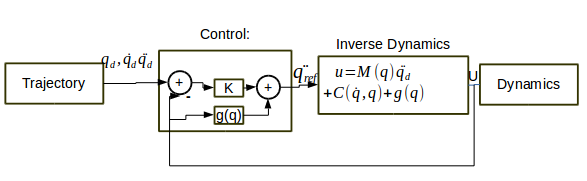
\includegraphics[width=0.7\textwidth]{img/2b.png} 
				\end{center}
				
				$\ddot{{q}}_{ref}={\ddot{q}}_d+K_D(\dot{q}_{des}-\dot{q})+K_P(q_{des}-q)+g(q)$
	\end{answer}
		
	\end{question}
	
	%----------------------------------------------
	
	\begin{question}{Comparison of Different Control Strategies}{12}
		In the following exercise you will investigate the differences of the following control algorithms, P, PID, PD with gravity compensation, and full inverse dynamics.
		The double pendulum is initiated hanging down, with state $\vec{q_\textrm{start}}={[-\pi,0]}$. We simulate the system with a time-step $dt=0.002$ seconds using symplectic Euler integration and run the simulation for $t_\textrm{end}=3s$. 
		
		Implement the control laws by filling the skeleton file \texttt{my\_ctl.py}. Use the following feedback gains $K_P=60, K_D=10, K_I=0.1$ for the first joint and $K_P=30, K_D=6, K_I=0.1$ for the second one.
		The target state of the double pendulum is set to $\vec{q_\textrm{des}}={[-\pi / 2,0]}$. 
		
		Create (max. 4) plots that compare the different control strategies and analyze the results. It is your choice how to illustrate your results. In your analysis you should include a discussion on the overall performance of each controller. Which controllers manage to go to the desired point, and how does the choice of a controller affects the behavior of the second joint of the pendulum? Additionally discuss which controller you would choose and why. The provided code is able to generate plot but feel free to modify it if you like. Points will be deducted for confusing plots. Do not forget to include your source code in your solutions.
		
\begin{answer}
\begin{minipage}{0.7\textwidth}
	\begin{figure}[H]
		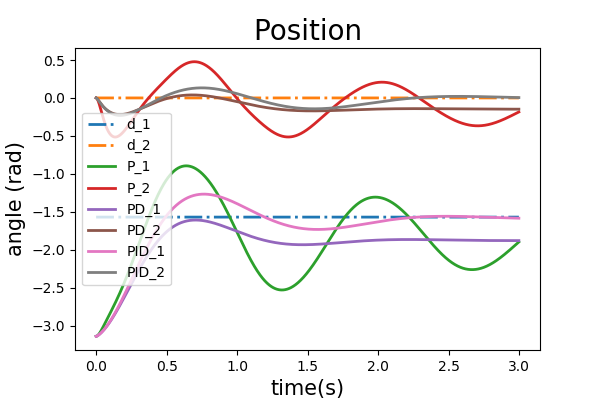
\includegraphics[width=1\textwidth]{img/2cpos1.png} 
		\caption{\label{fig:2cpos1} Comparing the position of the P,PD,PID controller}
	\end{figure}
\end{minipage} \hfill
\begin{minipage}{0.25\textwidth}
	First of all we compare the positioning behavior of the P,PD and PID controller. In figure \label{fig:2cpos1} we can see, that the P controller oscillates around the desired position. The PD controller has a steady state error. Only the PID controller behaves nicely and has no steady state error and does not overshoot the set point too much. Moreover the PID controller is not oscillating.
\end{minipage}

\begin{minipage}{0.7\textwidth}
	\begin{figure}[H]
		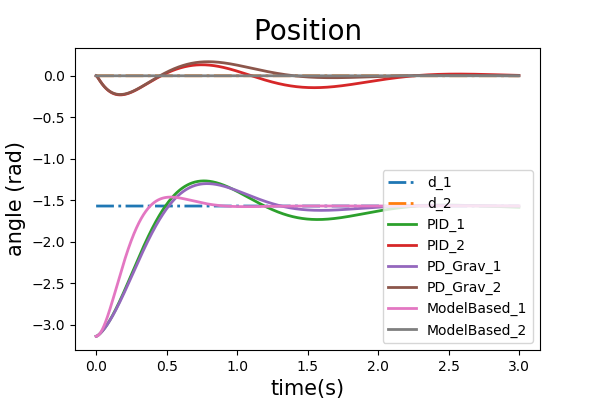
\includegraphics[width=1\textwidth]{img/2cpos2.png} 
		\caption{\label{fig:2cpos2} Comparison of the position of PID, PD\_GRAV and MPC}
	\end{figure}
\end{minipage} \hfill
\begin{minipage}{0.25\textwidth}
	The PD\_Grav. controller reaches the desired position of joint2 faster than the PID controller. However this costs a little bit more overshooting. Comparing all 3 controllers in figure \ref{fig:2cpos2} it is clear that the model based controller has the optimal positioning behavior. For joint1 it reaches the desired position quickest with minimal overshooting. In case of joint2 the model based controller is able to not oscillate at all.
\end{minipage}

\noindent\begin{minipage}{.5\textwidth}
	\centering
	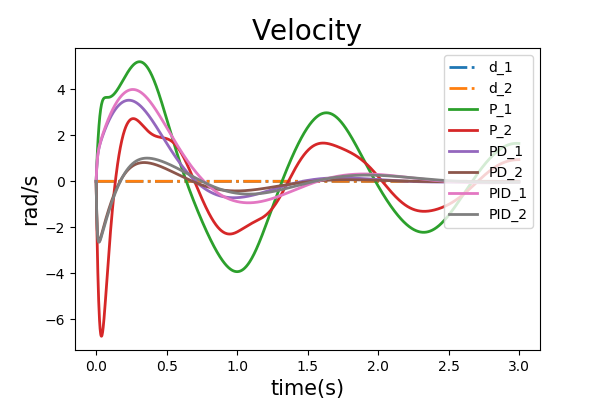
\includegraphics[width=1\textwidth]{img/2cvel1.png} 
	\captionof{figure}{Comparing the velocity of the P,PD,PID controller}
	\label{fig:2cvel1}            
\end{minipage}%
\begin{minipage}{.5\textwidth}
	\centering
	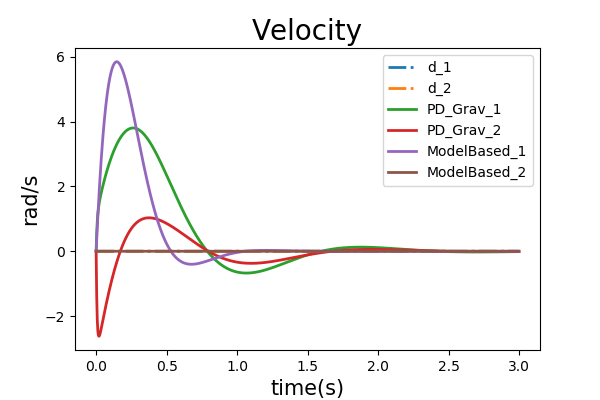
\includegraphics[width=1\textwidth]{img/2cvel2.png} 
	\captionof{figure}{Comparison of the velocity of PD\_GRAV and Model Based controller}
	\label{fig:2cvel2}               
\end{minipage}

Having a closer look to the velocity behavior of the controllers reveals that the all controllers (exept the P) reach the desired velocity of 0 rad/sec within 3 seconds. However again the model based controller is the fastest. 

In total it can be said the model based controller has the fastest positioning and velocity behavior of all controllers. Moreover it is the only one which is able to just stay at the desired position if the current position is equal to the desired position (see position for joint2). Neglecting any actuator saturation ("Stellgr\"ossenbeschr\"ankung") the model based controller is the best one. However if you have to care about an actor saturation you will probably not choose the model based controller, as it has the highest 
requirements on the actuators (see e.g. the high overshooting of the velocity (purpel line)). So if you have to care about actuator saturation the PD\_Grav is definitely better than the model based controller.

My\_clt.py:\\
\pythonexternal{src/myctl.py}

	\end{answer}

		
	
	\end{question}
	
	%----------------------------------------------
	
	\begin{question}{Tracking Trajectories}{4}
		Repeat the same experiment but this time use the provided time-varying target trajectory. Create (max 4) plots that compare the different control strategies and analyze the results. In your analysis discuss the overall performance and which controllers track the desired trajectory nicely. Additionally discuss which controller you would choose and why.
		
\begin{answer}
			\begin{minipage}{0.7\textwidth}
				\begin{figure}[H]
					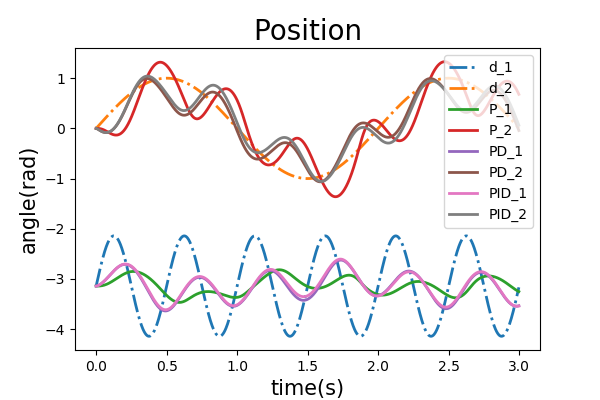
\includegraphics[width=1\textwidth]{img/2dpos1.png} 
					\caption{\label{fig:2dpos1} Comparison of the P,PD and PID positioning tracking behavior}
				\end{figure}
			\end{minipage} \hfill
			\begin{minipage}{0.25\textwidth}
				In figure \ref{fig:2dpos1} you can see that the tracking behavior of the P,PD,PID controllers fails. The desired positions of joint1 cannot be reached. Especially for joint1 we also can see that there is a time offset between the desired trajectory and the actual trajectories of the controllers.
			\end{minipage}
	
				\begin{minipage}{0.7\textwidth}
					\begin{figure}[H]
						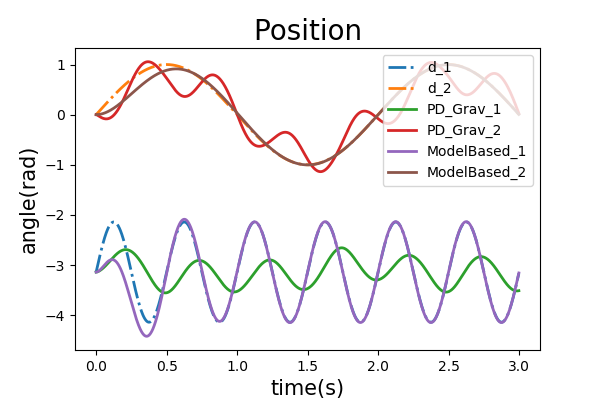
\includegraphics[width=1\textwidth]{img/2dpos2.png} 
						\caption{\label{fig:2dpos2} Comparison of the PD\_Grav. and model based controller's positioning tracking behavior}
					\end{figure}
				\end{minipage} \hfill
				\begin{minipage}{0.25\textwidth}
					In figure \ref{fig:2dpos2} you can see that the tracking behavior of the PD\_Grav and model based controllers differs a lot. The desired positions of joint1 and joint2 can only be reached by the model based controller. The PD\_Grav controller is faster than the P,PD,PID controller, however not fast enough to track the desired position of joint1 and joint2. It has a time offset and also does not reach the desired positions (see especially for joint1 green line).
				\end{minipage}
				
				\noindent\begin{minipage}{.5\textwidth}
					\centering
						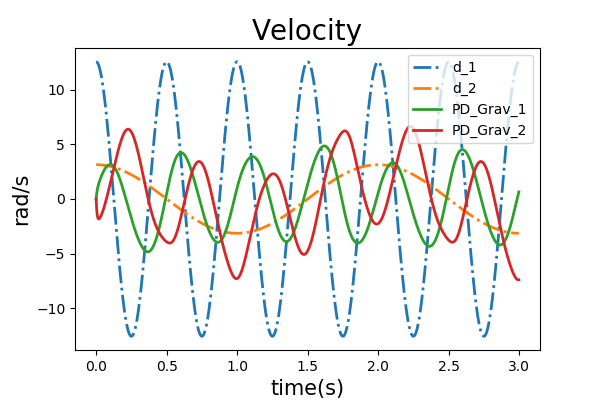
\includegraphics[width=1\textwidth]{img/2dvel1.png} 
					\captionof{figure}{The PD\_Grav tracking velocity behavior}
					\label{fig:2dvel1}            
				\end{minipage}%
				\begin{minipage}{.5\textwidth}
					\centering
					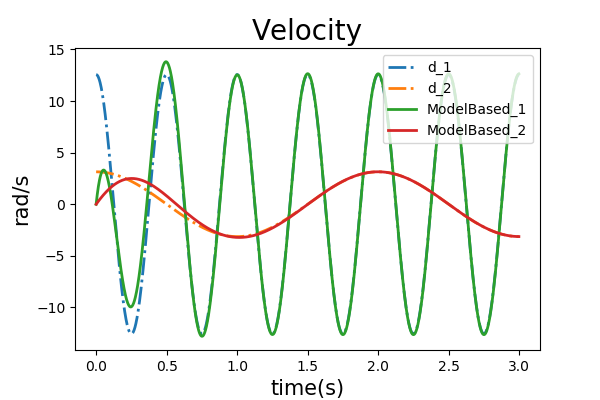
\includegraphics[width=1\textwidth]{img/2dvel2.png} 
					\captionof{figure}{The model based controller's velocity tracking behavior}
					\label{fig:2dvel2}               
				\end{minipage}
				
				Having a look at the two best positioning tracking controller's (the PD\_Grav and the model based) reveals, that their velocity tracking behavior also differs a lot. In \ref{fig:2dvel2} you can see that the velocity tracking behavior of the model based controller works perfectly well (with zero offset after some time), whereas the velocity behavior of the PD\_Grav controller fails (see \ref{fig:2dvel1}). In terms of tracking a trajectory the model based controller must be chosen, cause it is the only controller of the compared ones which is able to track a trajectory with zero offset. To track a trajectory a controller is required to reach a desired point fast enough with zero offset. This requirement is especially met by the model based controller.
	\end{answer}
		
	\end{question}
	
	%----------------------------------------------
	
	\begin{question}{Tracking Trajectories --- High Gains}{4}
		Repeat the same experiment (using the provided trajectory) but this time multiply the gains by ten. Create plots that compare the different control strategies and analyze the results. In your analysis discuss the overall performance and compare it to the previous case. Are there any drawbacks of using high gains?
		
\begin{answer}
	$K_{P,new}=K_{P,old}*10=[600,300]^T$ \\
	$K_{I,new}=K_{I,old}*10=[1,1]^T$\\
	$K_{D,new}=K_{D,old}*10=[100,60]^T$
	
					\noindent\begin{minipage}{.5\textwidth}
						\centering
						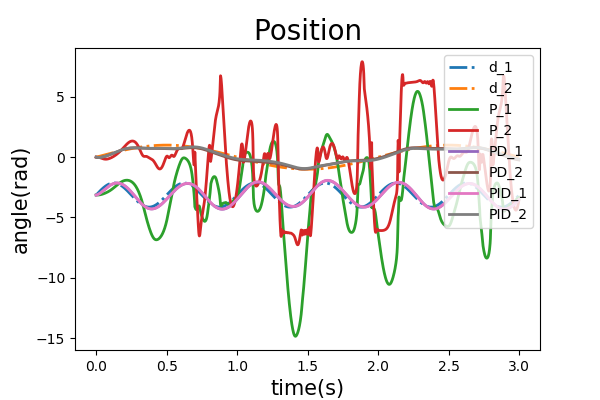
\includegraphics[width=1\textwidth]{img/2epos1.png} 
						\captionof{figure}{P,PD,PID position tracking behavior with high gains}
						\label{fig:2epos1}            
					\end{minipage}%
					\begin{minipage}{.5\textwidth}
						\centering
						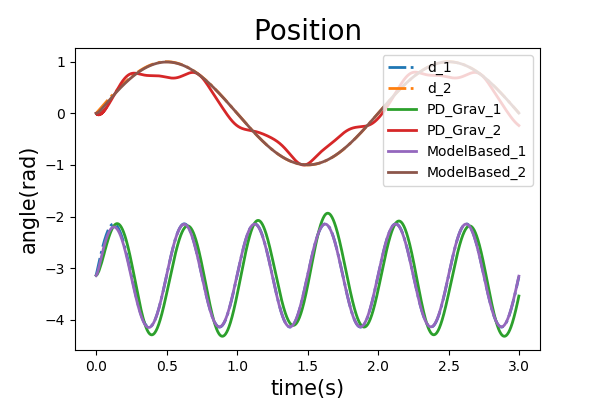
\includegraphics[width=1\textwidth]{img/2epos2.png} 
						\captionof{figure}{PD\_Grav, Model based position tracking behavior with high gains}
						\label{fig:2epos2}               
					\end{minipage}
	Having a look at figure \ref{fig:2epos1} one can see, that higher gains improve the positioning tracking behavior of the PD and PID controller. However the P controller's tracking behavior is worse (compared to d) ) cause it shows unstable behavior. So it can be concluded that higher gains might destabilize a system. The PD and PID controller however work better(compared to d) ), because increasing their gains results in a faster step response and now both controllers are fast enough to track the desired trajectory. Due to the derivative part these two controllers are also stable. Having a close look on the PD and PID controllers one can investigate that both have still a small time offset. 
	
	Having a look at figure \ref{fig:2epos2} one can see, that (neglecting any noise increasing effects and actuators saturation levels) the model based controller still behaves best. It as almost zero time offset and tracks the desired position for both joints perfectly. The PD\_Grav. PD and PID controllers behave all very similar. All have a small time offset and the small positioning errors of joint1 are even increased for tracking positioning accuracy of joint2.
	
	In total it should be said, that when using higher gain's the stability of the system has to be rechecked and also the actuators saturation level. Moreover increasing especially the K\_D's gain results in the fact, that the noise of a system is also increased.
	For this reason it is in general dangerous to higher the gain's too much.
	
	Neglecting any actuators saturation level's the Model based controller still has the best positioning tracking performance and should therefore be chosen.
	
	\end{answer}
		
	\end{question}
	
	%----------------------------------------------
	
	\begin{question}[bonus]{Task Space Control}{5}
		The robot must now reach a desired position in task space $\vec{x_\textrm{end}}={[-0.35,1.5]}$. In class we derived the Jacobian transpose, Jacobian pseudo-inverse, and Jacobian pseudo-inverse with damping methods. All of them are implemented in \texttt{my\_taskSpace\_ctl.py}. You are asked to implement also the null-space task prioritization method with a null-space resting posture $\vec q=[0,\pi]$. Run the simulation and plot the initial and final configuration of the robot. Then, change the resting posture to $\vec q=[0,-\pi]$ and redo the plots. Analyze in a couple of sentences your observation. Use the same damping coefficient $10^{-6}$ and include a code snippet to your solutions.
		
\begin{answer}
	Note: \\
{\footnotesize 	Task space is the cartesian space where the operation of robot is required. It has X,Y and Z ortho normal axes and Roll, Pitch and Yaw rotations about each axes. In other words, it is the space in which we live.}\\ \\
{\footnotesize 	Joint/Configuration space as the name suggests describes a particular configuration of robot or also called Posture. These postures are defined by individual and independent actuation of the joints. That means, it is those joints (revolute, prismatic, spherical, cylindrical etc.,) which do not depend on any other joint. The other name of the NUMBER that signifies the independency which describes the posture of the robot in concrete terms is called Degrees of Freedom.}


		
			\noindent\begin{minipage}{.5\textwidth}
				\centering
				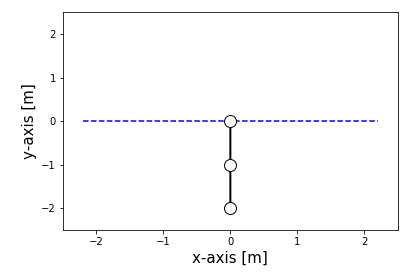
\includegraphics[width=1\textwidth]{img/2finitialpos.png} 
				\captionof{figure}{Task Space Control: Initial Position}
				\label{fig:2f3}            
			\end{minipage}%
			\begin{minipage}{.5\textwidth}
             Comparing the actual end position with the desired end position(-0.35,1.5) in task space:\\
             \begin{tabular}{ l l l }
             	method & endx & endy \\
             	JacTrans & -0.366 & 1.476 \\
             	JacPseudo &  0.137 & 1.1264 \\
             	JacDPseudo & -0.326 & 1.512 \\
             	JacNullSpace[0,pi] & -0.3247 & 1.512 \\
             	JacNullSpace[0,-pi] & -0.2985 & 1.4905 \\
             \end{tabular}
			\end{minipage}


			\noindent\begin{minipage}{.5\textwidth}
				\centering
				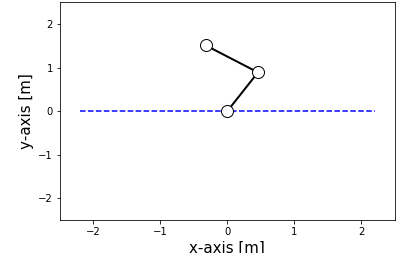
\includegraphics[width=1\textwidth]{img/2f0pi.png} 
				\captionof{figure}{Task Space Control Jac Null Space with resting pose [0,pi]}
				\label{fig:2f1}            
			\end{minipage}%
			\begin{minipage}{.5\textwidth}
				\centering
				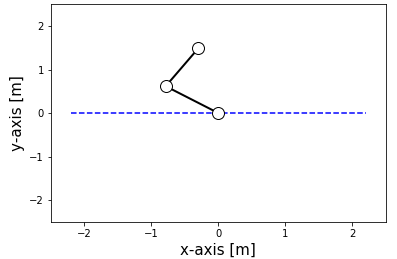
\includegraphics[width=1\textwidth]{img/2f0-pi.png} 
				\captionof{figure}{Task Space Control Jac Null Space with resting pose [0,-pi]}
				\label{fig:2f2}                 
			\end{minipage}

Using the JacDPseudo method the desired position is almost reached. However using the JacNullSpace method the desired position is approximated in two different ways one from the "left" (see \ref{fig:2f1}) and one from the right (see \ref{fig:2f2})

My\_taskspace.py:\\
\pythonexternal{src/mytaskspace.py}
	
	
	\end{answer}
		
	\end{question}
	
\end{questions}


	
	


\exercise{Machine Learning in a Nutshell}
For this exercise you will use a dataset, divided into training set and validation set (both attached). The first row is the vector $\vec x$ and the second row the vector $\vec y.$
\\
Based on these data, we want to learn a function mapping from $\vec x$ values to $\vec y$ values, of the form $\vec y=\vec{\theta}^{T}\vec{\phi}(\vec x)$.

For all questions requiring a plot, you also have to provide a snippet of your code!

You are allowed to use \texttt{scipy.spatial.distance.cdist} and \texttt{scipy.exp}.

\begin{questions}
	
	%----------------------------------------------
	
	\begin{question}{Supervised vs Unsupervised Learning}{2}
		Briefly explain the differences between supervised and unsupervised learning. 
		Is the above a supervised or unsupervised learning problem? Why?

\begin{answer}
		\begin{large}
			Supervised(predictive) Learning ("\"Uberwachtes Lernen"):
		\end{large}
	\\Predict unknown values. The given data actually has a label already. Each datapoint of the given data has an input and an output value:
	$f(\mathbf{X})=\mathbf{y}$ \\
	 Examples are Regression and Classification.
	\newline
	\newline
	\begin{large}
		Unsupervised(descriptive) Learning:
	\end{large}
	\\Understand given data.Find structures in data. This means labels have to be found first!
	Examples are Clustering, Dimensionality Reduction,Density Estimation.
	\\ 
	\\
	In the given example we have already the "labels": We have for each \textbf{x} an \textbf{y}. For this reason it is supervised learning.
	
	See also \hyperlink{http://oliviaklose.azurewebsites.net/machine-learning-2-supervised-versus-unsupervised-learning/}{http://oliviaklose.azurewebsites.net/machine-learning-2-supervised-versus-unsupervised-learning/}
	\end{answer}
	\end{question}
	%----------------------------------------------
	\begin{question}{Regression vs Classification}{2}
		Supervised learning is typically divided into regression and classification tasks. 
		Briefly explain what are the differences between regression and classification.

\begin{answer}
					\begin{large}
						Regression:
					\end{large}
					\\Regression algorithms are algorithms that learn to predict the value of a real function for a single instance of data. Regression algorithms can incorporate input from multiple features, by deterng the contribution of each feature of the data to the regression function. 
					
					Once the regression algorithm has trained a function based on already labeled data, the function can be used to predict the label of a new (unlabeled) instance. For example, a housing price predictor might use a regression algorithm to predict the value of a particular house, based on historical data about regional house prices.
					
					Examples:\\
					\begin{tabular}{l l }
						Bayesian Linear Regression & Creates a Bayesian linear regression model\\
						Boosted Decision Tree Regression & Creates a regression model using the Boosted Decision Tree algorithm \\
						Linear Regression & Creates a linear regression model \\
						Neural Network Regression & Creates a regression model using a neural network algorithm \\
						
					\end{tabular}
					
					\begin{large}
						Classification:
					\end{large}
					\\Is a method in machine learning of using data to determine the category, type, or class of an item or row of data. 
	\end{answer}
	\end{question}
	
	
	%----------------------------------------------
	
	\begin{question}{Linear Least Squares}{4}
		Consider the training set above to calculate features $\vec{\phi}(x)$ of the form $[\sin(2^{i}x)]_{i = 0 \ldots n-1}$. 
		Compute the feature values when $n$ is 2, 3 and 9 (i.e., when using 2, 3 and 9 features). 
		Use the linear least squares (LLS) method to predict output values $y$ for input values $x\in\{0, 0.01, 0.02, \ldots, 6\}$ using the different numbers of features. 
		Attach a single plot showing the three resulting predictions when using 2, 3 and 9 features (i.e., having $x$ and $y$ as axes).
		
	\begin{answer}
	Some Theory(LLS) (example for 2 Features): \\
	$x = (A^T A)^{-1} A^T b \quad \qquad$ 
	$\phi(x)=a_0 sin(x)+a_1 sin(2x) \qquad \qquad$
	$A=\begin{bmatrix}sin(x_1) & sin(2 x_1) \\ sin(x_2) & sin(2 x_2)\\ ...&...\\sin(x_n) &sin(2*x_n)\\ \end{bmatrix} x=\begin{bmatrix} a_0 \\ a_1 \end{bmatrix},b=\begin{bmatrix} y_0 \\...\\ y_n \end{bmatrix}$
	
	In the notation of this lecture:\\
	$y_i = \phi (x_i)^T \vec{\Theta}+\epsilon, \quad Parameters: \Theta = \begin{bmatrix}
	a_0\\...\\ a_n
	\end{bmatrix},\quad Features:\phi (x_i)=\begin{bmatrix}
	sin(x)\\...\\sin(2^n x)
	\end{bmatrix}, \Phi=[\phi_1, ..., \phi_n]^T, Y = [y_1, ..., y_n]^T, \quad \Theta = (\Phi^T \Phi)^{-1} \Phi^T Y$
	
	\begin{center}
		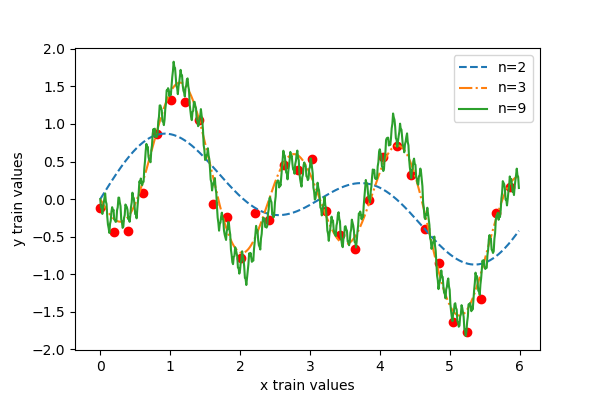
\includegraphics[width=0.7\textwidth]{img/3c.png} 
	\end{center}
	
	\pythonexternal{src/a13c.py}
	\end{answer}
		
	\end{question}
	
	
	%----------------------------------------------
	
	\begin{question}{Training a Model}{2}
		The root mean square error (RMSE) is defined as $\text{RMSE} = \sqrt{\frac{1}{N}\sum_{i=1}^{N}(y^{\text{true}}_i-y^{\text{predicted}}_i)^{2}}$, where $N$ is the number of data points. 
		Using the LLS algorithm implemented in the previous exercise, train a different model for each of the number of features between 1 and 9, i.e.,  [1,2,3...,9].
		For each of these models compute the corresponding RMSE for the training set. 
		Attach a plot where the x-axis represents the number of features and the y-axis represents the RMSE.
		
\begin{answer}
	\begin{center}
		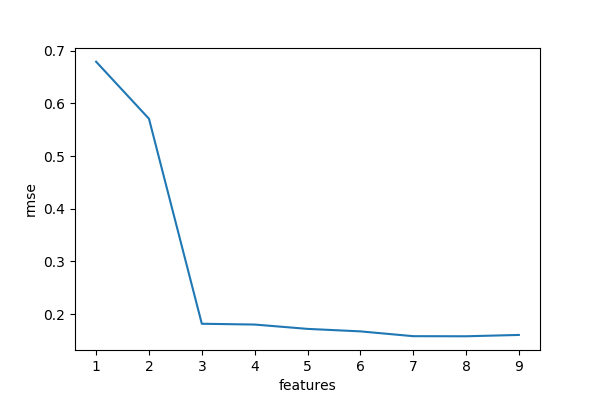
\includegraphics[width=0.5\textwidth]{img/3d.png} 
	\end{center}
	
		\pythonexternal{src/a13d.py}	
\end{answer}
		
	\end{question}
	
	
	%----------------------------------------------
	
	\begin{question}{Model Selection}{4}
		Using the models trained in the previous exercise, compute the RMSE of each of these models for the validation set.\\
		Compare in one plot the RMSE on the training set and on the validation set. 
		How do they differ? 
		Can you explain what is the reason for these differences? (Hint: remember the plot from Exercise~c)~) 
		What is the number of features that you should use to achieve a proper modeling?
		
	\begin{answer}
	Note: Use the parameters $a_i$ from c) on the validation dataset!
\begin{figure}[H]
	\centering
	\begin{minipage}{.5\textwidth}
		\centering
		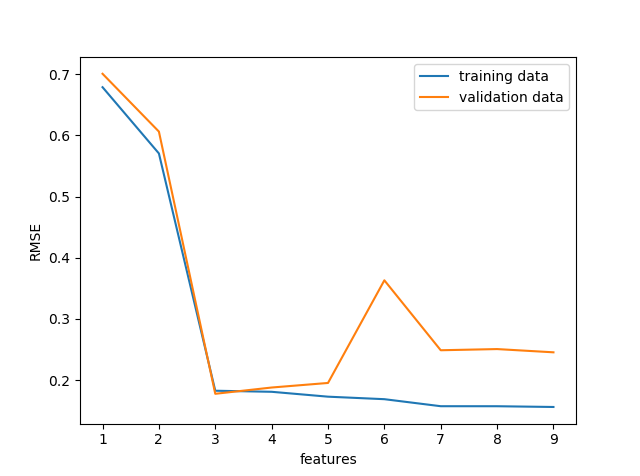
\includegraphics[width=1\textwidth]{img/3e.png} 
		\captionof{figure}{Comparing RMSE }
		\label{fig:test1}
	\end{minipage}%
	\begin{minipage}{.5\textwidth}
		\centering
		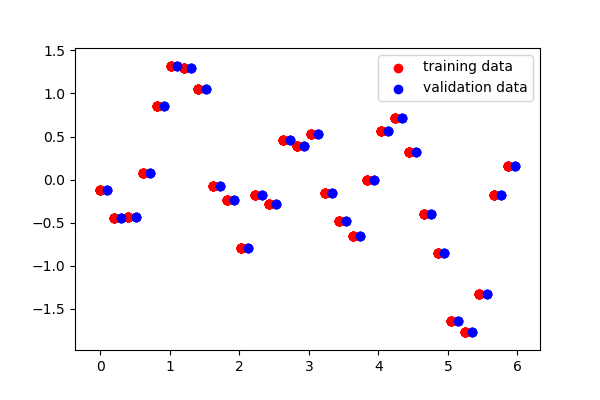
\includegraphics[width=1\textwidth]{img/data.png} 
		\captionof{figure}{Data sets}
		\label{fig:test2}
	\end{minipage}
\end{figure}

	
	How do they differ:\\
	Using 3 features the training set and the validation set have have the same rmse. Afterwards the rmse of the training set is marginally decreasing and the rmse of the validation set is increasing. 
	
	What is the reason for these differences:\\
	Using three features the model is sufficiently described (see e.g c). If you use more features the model is overfitted. Thus the rmse is increasing
	
	
	What is the number of features that you should use to achieve a proper modeling:\\
	As you can see in figure 29 the smallest rmse is reached for 3 features. For this reason 3 features should be used.

	\pythonexternal{src/a13e.py}
	\end{answer}
	\end{question}
	
	%----------------------------------------------
	
	\begin{question}{Cross Validation}{8}
		$K$-fold cross validation is a common approach to estimate the test error when the dataset is small.
		The idea is to randomly divide the training set into $K$ different datasets.
		Each of these datasets is then used as validation set for the model trained from the remaining $K-1$ datasets.
		The resulting vector of errors $\vec E = [ e_1... e_K ]$ can now be used to compute a distribution (typically by fitting a Gaussian distribution).
		When $K$ is equal to the number of data points, $K$-fold cross validation takes the name of leave-one-out cross validation (LOO).
		
		Apply LOO using only the training set and compute the mean/variance of the RMSE for the learned models. 
		Repeat for the models with the number of features between 1 and 9, i.e.,  [1,2,3...,9]
		
		Attach a plot showing the mean/variance (as a distribution) of the RMSE computed using LOO and having on the x-axis the number of features and on the y-axis the RMSE.
		Which is the optimal number of features now? 
		Discuss the results obtained and compare against model selection using train/validation set.
		
\begin{answer}
	\begin{center}
		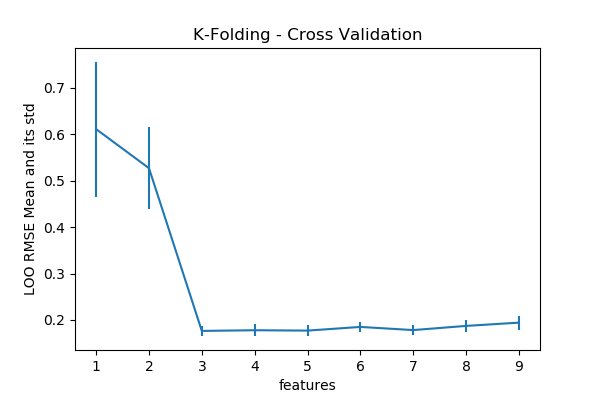
\includegraphics[width=0.7\textwidth]{img/3f.png} 
	\end{center}
	
	\pythonexternal{src/a13f.py}

	
	\end{answer}
	\end{question}
	
	
	
	%----------------------------------------------
	
	
	\begin{question}{Kernel Functions}{2}
		A kernel function $k(\vec{\mbox{x}}_{i},\vec{\mbox{x}}_{j})$ is given by the inner product of two feature vectors. Write out the kernel function for the previous set of features where $n=3$.
		
	\begin{answer}
	
		$k(x_i,x_j)_{n=3}=\begin{bmatrix}
		sin(x_i)&sin(2x_i)&sin(4x_i)
		\end{bmatrix}
		\begin{bmatrix}
			sin(x_j)\\sin(2x_j)\\sin(4x_j)
		\end{bmatrix}=sin(x_i)sin(x_j)+sin(2x_i)sin(2x_j)+sin(4x_i)sin(4x_j)$

	References:\\
	\hyperlink{https://de.wikipedia.org/wiki/Kernel\_(Maschinelles\_Lernen)}{https://de.wikipedia.org/wiki/Kernel\_(Maschinelles\_Lernen)}
	
	\hyperlink{https://en.wikipedia.org/wiki/Kernel\_(statistics)}{		https://en.wikipedia.org/wiki/Kernel\_(statistics)}
	

	\end{answer}
	\end{question}
	
	
	%----------------------------------------------
	
	\begin{question}{Kernel Regression}{6}
		
		The kernel function in the previous question required explicit definition of the type and number of features, which is often difficult in practice. Instead, we can use a kernel that defines an inner product in a (possibly infinite dimensional) feature space. \\
		Using the training set and an exponential squared kernel 		$k( \vec{x}_{i} , \vec{x}_{j} )= \exp ( -\frac{1}{\sigma^{2}} \Vert \vec{x}_{i}-\vec{x}_{j}\Vert ^{2} )$ with $\sigma=0.15$, predict output values $y$ for input values $x\in\{0,0.01,\ldots,6\}$. Attach a plot of your results.
		\\
		(Hint: use standard kernel regression: $f(\mbox{\ensuremath{\vec{x}}})=\vec{k}\T\vec{K}^{-1}\vec{y}$ with $\vec{K}_{ij}=k(\vec{x}_{i},\vec{x}_{j})$ and $\vec{k}_{i}=k(\vec{x},\vec{x}_{i})$).
		
		Compute the RMSE on the validation set for the kernel regression model. Compare it with the RMSE of the best LLS model you found.
		
\begin{answer}
	Some Theory:
	\begin{itemize}
		\item squared Euclidean distance: $|| a - b||^2 = \sqrt{ (a_1-b_1)^2+...+(a_n-b_n)^2}^2 =  (a_1-b_1)^2+...+(a_n-b_n)^2$
		\item Kernel function: $k(x_1,x_2)=\phi(x_1)^T \phi(x_2), \quad (\text{inner product})$
		\item Kernel regression: $y_{pred} = f(x_{\text{pred}})=k^T_{\text{pred, dataset}} K^{-1}_{\text{dataset}} y_{\text{dataset}}$
		\item $k_i=k(x,x_i)=[e^{- \frac{||x_{pred}- x_{0,dataset} ||^2}{\sigma^2}}, ... ,e^{- \frac{||x_{pred}- x_{n,dataset} ||^2}{\sigma^2}}], \quad \text{Gaussian Radial Basis kernel function} $
		\item $K_{ij}=k(x_i,x_j)=\begin{bmatrix}
		e^{- \frac{||x_{0,dataset}- x_{0,dataset} ||^2}{\sigma^2}}&...&e^{- \frac{||x_{n,dataset}- x_{0,dataset} ||^2}{\sigma^2}}\\...&...&...\\e^{- \frac{||x_{0,dataset}- x_{n,dataset} ||^2}{\sigma^2}}&...&e^{- \frac{||x_{n,dataset}- x_{n,dataset} ||^2}{\sigma^2}}
		\end{bmatrix}$
	\end{itemize}
	\begin{figure}[H]
		\centering
		\begin{minipage}{.5\textwidth}
			\centering
				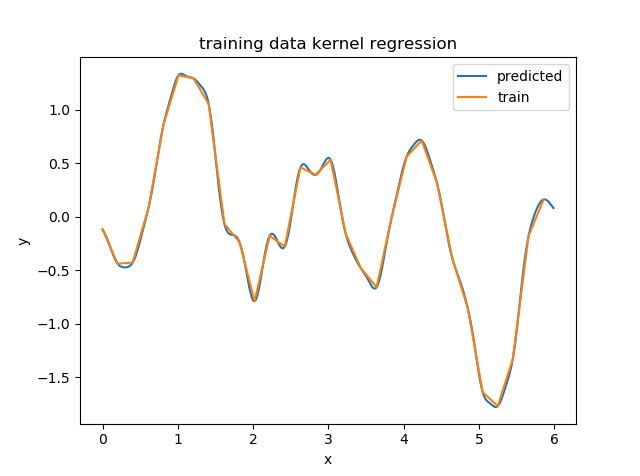
\includegraphics[width=1\textwidth]{img/3g.png} 
		\end{minipage}%
		\begin{minipage}{.5\textwidth}
			\centering
			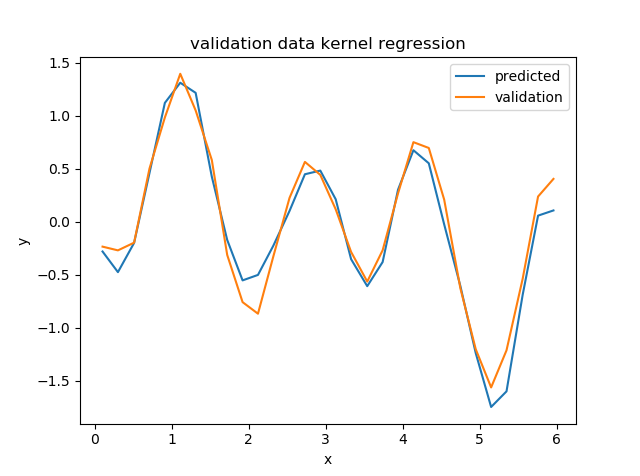
\includegraphics[width=1\textwidth]{img/3g2.png} 
		\end{minipage}
	\end{figure}
	
	
		The prediction for the training data is nearly perfect. You can see no difference between the prediction and the rail data. But th prediction for the validation data is not so well, you can see big differences for $x=2$. The calculated RMSE is 0.2422. So it is slightly bigger compared to the Linear Regression model with three features.
		
		\pythonexternal{src/a13g.py}
	
	Refererences:\\
	\url {https://en.wikipedia.org/wiki/Radial_basis_function_kernel}
	
	\end{answer}
	\end{question}
	
	
	%----------------------------------------------
	
	\begin{question}[bonus]{Derivation}{5}
		Explain the concept of ridge regression and why/when it is used.
		Derive its final equations presented during the lecture.\\
		(Hint: remind that for normal linear regression the cost function is $J = \frac{1}{2}\sum_{i=1}^N ( f(\vec x_i) - y_i ) ^2 \,$ )\\
		(Hint 2: use matrix notation)
		
\begin{answer}
		
		Ordinary Linear Squares (OLS):
		\begin{itemize}
			\item Parameters $\Theta$ are Best linear unbiased estimators (BLUE).
			\item The Parameters have the smallest variance out of all other unbiased estimators.
			\item If 2 or more parameters are highly correlated the variance is quite high and quite different solution's occur for different data sets. In such a case Ridge Regression should be used! 
			\item $f_{\Theta}=\phi^T(x_i) \Theta$
			\item $J=\frac{1}{2} \sum_{i=1}^{N} (y_i - f_{\Theta}(x_i))^2, \quad J=\frac{1}{2}(Y-\Phi \Theta)^T (Y-\Phi \Theta)$
			\item $\Theta = (\Phi^T \Phi)^{-1} \Phi^T Y$
		\end{itemize}
		\bigskip
		Ridge ("Kamm") Regression:
		\begin{itemize}
			\item Estimators are biased and can therefore have an even lower variance compared to OLS.
			\item Especially if the parameters are highly correlated ridge regression is a powerful method to restrict the correlation of the parameters using a 
			lagrangian multiplier $\lambda$.
			\item $min_\Theta ||y-\Phi \Theta||^2_2+\lambda ||\Theta||^2_2 $
			\item $J=\frac{1}{2} [ \sum_i^N (y_i \phi(x_i) \Theta)^2+\lambda \Theta^T \Theta], \quad J=\frac{1}{2}[(Y-\Phi \Theta)^T (Y-\Phi \Theta)+\lambda \Theta^T \Theta],\quad \frac{\partial J}{\partial \Theta}=0$
			\item $J=\frac{1}{2}[Y^T Y-Y^T \Phi \Theta - \Phi^T \Theta^T Y + \Phi^T \Theta^T \Phi \Theta+\lambda \Theta^T \Theta] = \frac{1}{2}[Y^T Y-2Y^T \Phi \Theta+ \Phi^T \Theta^T \Phi \Theta+\lambda \Theta^T \Theta]$
			\item $\frac{\partial J}{\partial \Theta}=Y^T \Phi - \Phi^T \Phi \Theta +\lambda \Theta = 0, \quad \Phi^T Y = (\Phi^T \Phi + \lambda I) \Theta$
			\item $\Theta = (\Phi^T \Phi+\lambda I)^{-1} \Phi^T Y$
		\end{itemize}
		
				\begin{center}
					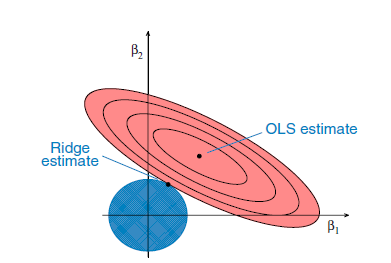
\includegraphics[width=0.7\textwidth]{img/ridge.png} 
				\end{center}

		
		\url{https://www.youtube.com/watch?v=5asL5Eq2x0A}\\
		\url{https://onlinecourses.science.psu.edu/stat857/node/155}
	\end{answer}
	
	
	\end{question}	
	
\end{questions}


	
\end{document}

